\subsection{Angriffsmöglichkeiten in einem geswitchten Netzwerk}
\label{sec:geswitchtes_netz}

\subsubsection{MAC-Flooding}
Der Speicher der Switch-Tabelle ist begrenzt. MAC-Flooding macht sich das zunutze. Der Switch wird mit gefälschten MAC-Adresse überhäuft, bis der Speicher der Tabelle voll ist.
Dann verhält sich der Switch wie ein Hub, was auch Ziel des Angriffes ist.

Einige Switches haben Schutzmaßnahmen gegen diesen Angriff, diese sind allerdings eher in den höheren Preiskategorien zu finden. Zum Beispiel kann für einen Port eine Liste mit zugelassenen MAC-Adressen angelegt werden. Frames von nicht bekannten MAC-Adressen werden verworfen, bzw. der betroffene Port wird gesperrt.

\subsubsection{MAC-Spoofing}
Eine weitere Möglichkeit, als Dritter den Datenverkehr mitzulesen, nennt sich MAC-Spoofing. Hierbei wird die Quell-Adresse mit der MAC-Adresse des Angreifers ersetzt. Die Respons des Empfängers des Frames wird an den Angreifer gesendet. Somit können die Daten vom Angreifer mitgelesen werden, ohne dass der eigentliche Sender und auch der Empfänger etwas davon mitbekommen. Der Angreifer wird allerdings in die Switch-Tabelle eingetragen. Diesen Umstand kann man nutzen und den Angriff umgehen, indem man wie oben schon erwähnt eine Liste mit erlaubten MAC-Adresse für den jeweiligen Post erstellt.

\subsubsection{ARP-Spoofing}
Das ist ein interessanter Angriff, denn er nutzt eine Schwäche des ARP-Protokolls aus.
Dazu wird kurz erklärt, wofür das ARP-Protokoll da ist und wie es funktioniert.
\\ \\
Das ARP-Protokoll dient zur Auflösung von IP-Adresse zu zugehöriger MAC-Adresse in einem lokalen Netzwerk.
Jeder Netzwerkteilnehmer kennt dieses Protokoll und jeder Teilnehmer verfügt auch über eine ARP-Tabelle, in welcher die ihm bekannten Teilnehmer mit IP-Adresse und zugehöriger MAC-Adresse hinterlegt sind. Das ist notwendig, um die Pakete, die z.B. über IPv4 versendet werden, über die einzelnen Komponenten im Netzwerk weiterzuleiten, d.h.: versendet mein Rechner eine Anfrage nach außen, z.B. ein Aufruf der Seite www.hm.edu, so steht in Header der Schicht 3 die IP-Adresse des geforderten Servers. Auf Schicht 2 werden immer MAC-Adressen benötigt, um zum nächstmöglichen Gerät zu senden. In meinem Heimnetzwerk wäre das z.B. ein Router, denn es wurde ja eine externe IP-Adresse aufgerufen, kein intern bekanntes Geräte wie z.B. ein Drucker. Der Rechner kennt den Router bereits, und weiß, dass er diesen wählen muss, wenn eine externe IP-Adresse angefragt ist. Somit wählt er die MAC-Adresse des Routers und sendet die Frames an diese Adresse.
\begin{figure}
	\centering
	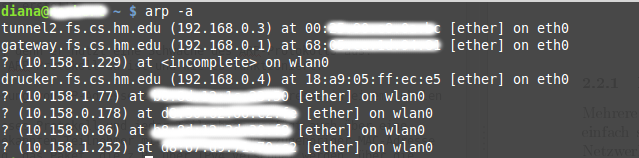
\includegraphics[width=1\linewidth]{images/arp-tabelle.png}
	\caption{Auszug aus einer ARP-Tabelle, MAC-Adressen entfernt}
\end{figure}

Damit sich alle Rechner in einem Netzwerk kennen, wird in regelmäßigen Abständen eine Broadcast-Nachricht, ein sogenannter ARP-Request, gesendet, um zu ermitteln, welche MAC-Adresse zu einer IP-Adresse gehört und diese auch aktuell zu halten, damit keine Daten an Geräte gesendet werden, die sich eventuell gar nicht mehr im Netzwerk befinden. Somit kennen sich alle Geräte in einem internen Netzwerk.
\\
Das Protokoll hat zwei Schwäche, die von einem Angreifer ausgenutzt werden können.\cite[vgl.]{Psarros}
\begin{enumerate}
	\item Jede ARP-Response wird ausgewertet, auch wenn es gar keinen unmittelbaren Request gab
	\item Die Identität des Netzwerkteilnehmer wird nicht überprüft, es wird einfach angenommen, dass das Gerät korrekt funktioniert
\end{enumerate}

\subsection{Theoretisches Beispiel eines Angriffs mit ARP-Spoofing}
In einem Netzwerk befinden sich folgende Teilnehmer
\begin{itemize}
	\item Fabian
	\item Diana
	\item X
	\item Angreifer Y
\end{itemize}
Der Angreifer Y möchte den Datenverkehr von Fabian und Diana mitlesen und/oder verändern. Dafür muss er seine eigenen MAC-Adresse in die ARP-Tabelle von Fabian und Diana zu der jeweiligen IP-Adresse der Kommunikationspartner eintragen. Die ARP-Einträge von Fabian und Diana sehen dann wie folgt aus:
\vfill
\begin{tabular}{l c l}
	ARP-Tabelle von Fabian & & \\
	\hline
	IP-Adresse Diana & : & MAC-Adresse von Y \\
	IP-Adresse X & : & MAC-Adresse von X \\
	IP-Adresse Y & : & MAC-Adresse von Y \\
\end{tabular}
\vfill
\begin{tabular}{l c l}
	ARP-Tabelle von Diana & & \\
	\hline
	IP-Adresse Fabian & : & MAC-Adresse von Y \\
	IP-Adresse X & : & MAC-Adresse von X \\
	IP-Adresse Y & : & MAC-Adresse von Y \\
\end{tabular}
\vfill
Diese gefälschten Einträge in der ARP-Tabelle der Netzwerkteilnehmer kann man mit dem Werkzeug dsniff umsetzten, welche später genauer Beschreiben wird.

Sind die ARP-Tabllen zugunsten des Angreifers verändert, kann dieser nun den Datenverkehr von Fabian und Diana mitlesen, da Fabian die Pakte bzw. Frames für Diana an die MAC-Adresse des Angreifers senden wird, Diana die Frames für Fabian ebenfalls. Die Frames werden über den Switch an den Angreifer verteilt, Fabian und Diana erhalten diese nicht.
\begin{figure}
	\centering
	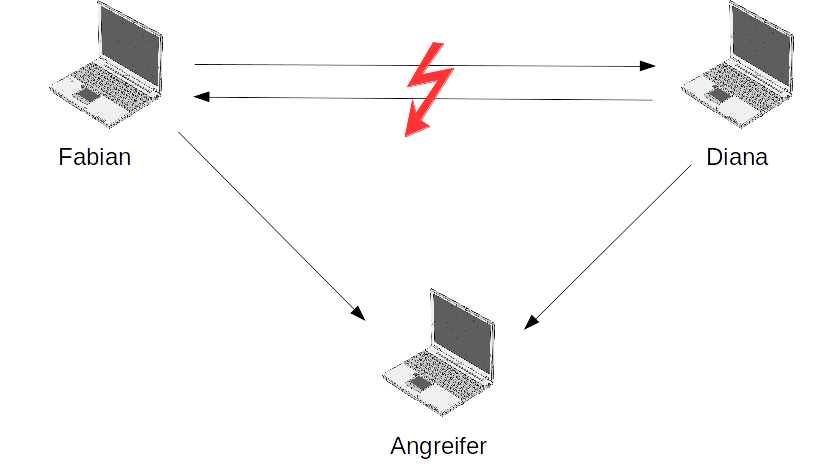
\includegraphics[width=1\linewidth]{images/ARP-Tabelle-manipuliert.png}
	\caption{Darstellung der Kommunikation nach erfolgreicher Manipulation der ARP-Tabellen \cite{ARP-Tabelle-Bild-1}}
\end{figure}
Dies gilt für geswitchte Netzwerke ebenso wie für Netzwerke, in welchem ein Hub eingesetzt ist. Diana und Fabian würden in diesem Fall zwar die Frames erhalten, diese allerdings verwerfen, da sie nicht für sie adressiert sind.

Zu diesem Zeitpunkt empfängt der Angreifer die Daten, die vermeintlich zwischen Fabian und Diana gesendet werden. Allerdings muss der Angreifer zudem dafür sorgen, dass Fabian und Diana die Frames erhalten, die erwartet werden, denn das Protokoll, dass für die Kommunikation darüber liegt, TCP, würde die Verbindung sonst abbrechen. Es würden keine Daten ausgetauscht werden, da somit schon der 3-Wege-Handshake des TCP-Protokolls scheitert.
Der Angreifer muss dafür sorgen, dass die Frames bzw. Pakete an den eigentlichen Empfänger weitergeleitet werden, damit die Verbindung bestehen bleibt. Dafür muss die MAC-Adresse des eigentlichen Empfängers in den Header eingetragen werden, damit der Empfänger die Pakete nicht verwirft. Dabei können die Daten vom Angreifer manipuliert oder analysiert werden. Der Angreifer kann das mit mehreren Möglichkeiten erreichen, z.B. mit IP-Forwarding. Wichtig ist dabei nur, dass die Verzögerung im Rahmen des Timeouts bleibt, da die Verbindung sonst abbrechen könnte.
\begin{figure}[H]
	\centering
	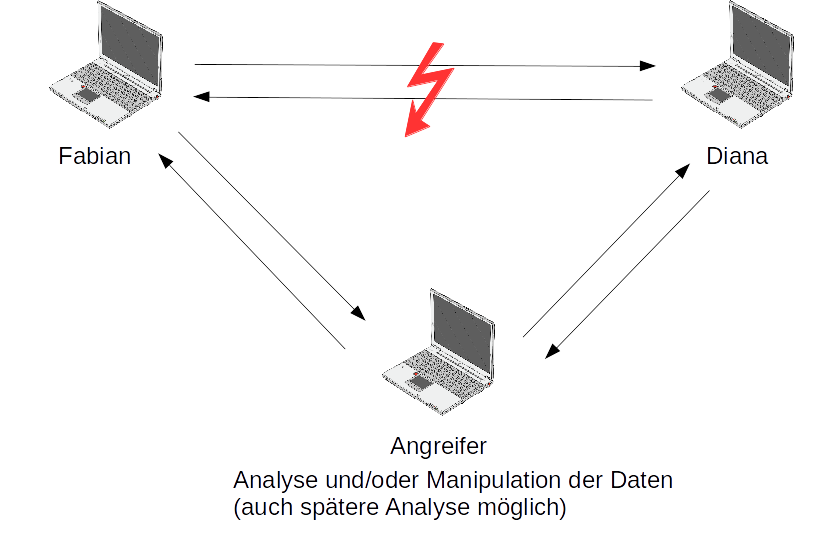
\includegraphics[width=1\linewidth]{images/ARP-Tabelle-manipuliert_1.png}
	\caption{Angreifer muss die abgefangenen Frames an den eigentlichen Empfänger weiterleiten, damit Verbindung aufrecht erhalten bleibt \cite{ARP-Tabelle-Bild-2} }
\end{figure}
Für die Analyse der abgefangenen Daten gibt es ebenfalls Werkzeuge, welche mit Filtern nach den gewünschten Informationen suchen.

\subsection{Werkzeug zur Umsetzung eines ARP-Spoofing-Angriffs}
Es gibt mehrere Werkzeuge, die sich gut dafür eigenen, hier wird dsniff näher erläutert \cite[vgl.]{dsniff_monkey}.

dsniff bietet eine Sammlung von Werkzeugen, mit welchen eine Man-in-the-middle-Attakte umgesetzt werden kann \cite[vgl.]{dsniff_beschreibung}. Unter anderen ist da der Passwort-Sniffer dsniff enthalten, welcher unverschlüsselte Passwörter im Netzwerk filtert.

arpspoof macht genau das, was oben beschreiben wurde. Dieses Werkzeuge leitet Pakete vom Zielhost, welchen in einem Netzwerk zu einem anderen Host gesendet werden sollen, um, indem die ARP-Antworten (ARP-Replies) vom Angreifer gefälscht werden.\cite[vgl.]{arpspoof}

Dazu kommen noch spezielle Sniffer wie urlsniff und mailsniff, und einiges mehr.
Für den einfachen Zweck und diesem theoretischen Beispiel würde arospoof ausreichen.

Im Anhang ist eine Auflistung aller enthaltener Werkzeuge mit Funktionalität aufgelistet.


\subsection{Schutzmaßnahmen und Kontrolle im Netzwerke}
Die einzig wirklich sichere Methode zur Vermeidung von ARP-Spoofing in einem Netzwerk ist die manuelle Verwaltung der IP- und zugehörigen MAC-Adressen.
Das bringt allerdings einiges an Arbeitsaufwand mit sich, und dieser steigt zudem mit jedem neuen Netzwerkteilnehmer. Gerade in einem Netzwerk mit wechselnden Geräten ist das fast nicht umsetzbar bzw. sehr unpraktisch.

Eine weitere Maßnahme wäre, den Netzwerkverkehr zu überwachen, z.B. am Switch, und auf eine erhöhte Anzahl an ARP-Responses zu achten. Häufen sich diese, könnte man einen Angriff verdächtigen und der Sache auf den Grund gehen.

Auch Arpwatch\cite{arpwatch-download} wäre ein Möglichkeit, um das Netzwerk vor einem solchen Angriff zu schützen. Wenn das Programm gestartet wird, werden alle ARP-Pakete im Netzwerk, welche an einem Rechner ankommen, mit den bereits bekannten MAC-Adressen abgeglichen. Diese Adressen sind in der Datei arp.dat hinterlegt und werden da verwaltet. Taucht eine nicht bekannte Adresse auf, wird ein Eintrag in den syslogs gemacht und eine Nachricht an den Benutzer oder root gesendet. Hat sich die Zuordung von MAC- und IP-Adresse geändert, wird ebenfalls ein Eintrag in den syslogs gemacht. \cite[vgl.]{arpwatch}
